\documentclass[14pt,aspectratio=169]{beamer}
\usepackage[T1]{fontenc}
\usepackage[utf8]{inputenc}
\usepackage{lmodern,booktabs,tikz}
\usetikzlibrary{arrows.meta,positioning}
\setbeamertemplate{navigation symbols}{}
\setbeamertemplate{footline}[frame number]
\setbeamercolor{structure}{fg=blue!55!black}
\setbeamercolor{alerted text}{fg=red!65!black}
\setbeamerfont{normal text}{size=\fontsize{14}{17}\selectfont}
\setbeamerfont{title}{size=\fontsize{22}{26}\selectfont}
\setbeamerfont{frametitle}{size=\fontsize{20}{24}\selectfont}
\setbeamerfont{author}{size=\fontsize{14}{17}\selectfont}
\setbeamerfont{institute}{size=\fontsize{14}{17}\selectfont}
\setbeamerfont{date}{size=\fontsize{14}{17}\selectfont}
\setbeamerfont{itemize/enumerate body}{size=\fontsize{14}{17}\selectfont}
\setbeamerfont{itemize/enumerate subbody}{size=\fontsize{14}{17}\selectfont}
\setbeamerfont{block title}{size=\fontsize{16}{19}\selectfont}
\setbeamerfont{block body}{size=\fontsize{14}{17}\selectfont}
\setbeamerfont{footline}{size=\fontsize{14}{17}\selectfont}
\setbeamersize{text margin left=8mm,text margin right=8mm}
\title{Auto-Assessment: Rubric-Grounded Grading of Handwritten Answer Sheets with Red-Ink Feedback}
\author{Basavaraj A Naduvinamani (DA25C005)}
\institute{DA7016, IIT Madras}
\date{}

\begin{document}

\begin{frame}
\titlepage
\end{frame}

\begin{frame}{The bar: marks that help a student improve}
\begin{itemize}
  \item Inputs: question paper, rubric, model answers and a sheet.
  \item Outputs: marks per question, evidence and a concrete next step.
  \item Automatic marking by default: no teacher action on each answer.
  \item Uncertain or flagged answers defer to a teacher; regrades allow appeal.
\end{itemize}
\begin{block}{Educational goal}
Feedback specific enough to improve. Learning gains are not yet measured.
\end{block}
\end{frame}

\begin{frame}{Pipeline: from a sheet to inspectable marks}
\centering
% Adapted from the report's figure: same stages, interfaces and serpentine flow.
% Explicit quote checking and the final advocate-only path suit the talk.
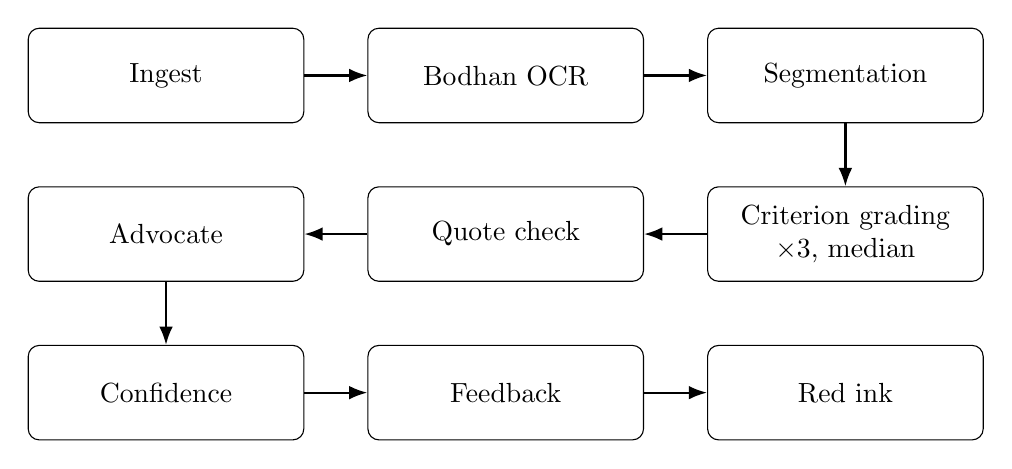
\begin{tikzpicture}[
  stage/.style={draw,rounded corners,align=center,minimum width=35mm,minimum height=12mm,font=\normalsize},
  flow/.style={-{Latex},thick},node distance=8mm and 8mm]
\node[stage] (ingest) {Ingest};
\node[stage,right=of ingest] (ocr) {Bodhan OCR};
\node[stage,right=of ocr] (segment) {Segmentation};
\node[stage,below=of segment] (grade) {Criterion grading\\$\times 3$, median};
\node[stage,left=of grade] (quote) {Quote check};
\node[stage,left=of quote] (advocate) {Advocate};
\node[stage,below=of advocate] (confidence) {Confidence};
\node[stage,right=of confidence] (feedback) {Feedback};
\node[stage,right=of feedback] (ink) {Red ink};
\draw[flow] (ingest)--(ocr);
\draw[flow] (ocr)--(segment);
\draw[flow] (segment)--(grade);
\draw[flow] (grade)--(quote);
\draw[flow] (quote)--(advocate);
\draw[flow] (advocate)--(confidence);
\draw[flow] (confidence)--(feedback);
\draw[flow] (feedback)--(ink);
\end{tikzpicture}

\end{frame}

\begin{frame}{What makes an award defensible?}
\begin{itemize}
  \item \textbf{Evidence:} verbatim quotes checked in code; unsupported awards are withdrawn. Marks stay within rubric bounds.
  \item \textbf{Deferral:} run spread, review changes and OCR concerns lower confidence and trigger teacher review.
  \item \textbf{Lenient policy:} credit valid ideas in other words; do not penalise spelling unless the rubric asks.
\end{itemize}
\begin{block}{Review default}
An advocate may recover missed credit with evidence. The lower-only critic is optional and off by default.
\end{block}
\end{frame}

\begin{frame}{Data: keep questions out of both splits}
\begin{itemize}
  \item \textbf{SPRAG:} 570 typed CS/ML/Python answers, 114 questions, marks 0--5; consensus of two independent graders. CC BY 4.0.
  \item \textbf{Question-level split:} dev 115 answers / 23 questions; test 455 / 91. Seed 0.
  \item \textbf{Handwritten classroom:} 9 students, 15 two-mark questions, 135 answers; one teacher, Bodhan OCR.
\end{itemize}
\begin{block}{Development discipline}
All prompt, policy and configuration choices on dev; test once per reported configuration.
\end{block}
\end{frame}

\begin{frame}{SPRAG test: beyond overlap, below human agreement}
\centering
\begin{tabular}{lrrr}
\toprule
System & QWK & MAE & Within 1 \\
\midrule
Lexical baseline & 0.375 & 1.62 & 40\% \\
Final: advocate only & 0.723 & 0.85 & 76\% \\
Human vs human & 0.962 & 0.22 & 100\% \\
\bottomrule
\end{tabular}
\begin{block}{Final configuration, test $n=455$}
QWK 0.723 [0.667, 0.773]; 95\% bootstrap clustered by question. MAE is in marks out of 5.
\end{block}
QWK uses half-mark bins. Human agreement is still much higher.
\end{frame}

\begin{frame}{A lower-only critic increases under-marking}
\centering
\begin{tabular}{lrrr}
\toprule
Dev configuration & QWK & MAE & Bias \\
\midrule
Full: advocate + critic & 0.675 & 1.01 & $-0.59$ \\
Critic only & 0.640 & 1.06 & $-0.77$ \\
Advocate only & 0.669 & 0.92 & $-0.05$ \\
No review & 0.681 & 0.96 & $-0.54$ \\
\bottomrule
\end{tabular}
\begin{block}{Choose on dev, not on the best test score}
Advocate-only: lowest MAE and near-zero bias. A critic can remove credit but cannot restore a missed valid idea.
\end{block}
Bias = system $-$ human. These ablation runs are separate from the headline run.
\end{frame}

\begin{frame}{Confidence: always read error with coverage}
\begin{block}{Full pipeline: advocate + critic}
Confidence $\geq 0.8$: \textbf{62\% auto-marked at MAE 0.66}. The rest go to the teacher.
\end{block}
\begin{block}{Final configuration: advocate only}
Same threshold: \textbf{92\% coverage at MAE 0.76}. Without critic disagreements, confidence separates difficulty less sharply.
\end{block}
Both results are on SPRAG test. Confidence is a diagnostic signal, not a calibrated correctness probability.
\end{frame}

\begin{frame}{Handwriting adds reading uncertainty}
\begin{itemize}
  \item Full pipeline with Bodhan OCR; 135 answers, one teacher.
  \item QWK \textbf{0.47 [0.32, 0.57]}, question-clustered interval; MAE \textbf{0.55 of 2}; bias \textbf{$-0.49$}.
  \item \textbf{75 of 135} flagged for review. OCR uncertainty and teacher credit for vague answers contribute to disagreement.
  \item Post-hoc offset: QWK 0.55 [0.44, 0.65], \textbf{item-level} interval; no claim of improved reasoning.
\end{itemize}
This measures the full pipeline, not the new advocate-only default. No second teacher provides a human--human ceiling.
\end{frame}

\begin{frame}{Injection can change marks; Indic support is a demo}
\begin{block}{Targeted injection check}
Before fix: \textbf{7 of 30} answers gained marks (mean $+0.17$ of 5); 3 reached full marks.
\end{block}
\begin{itemize}
  \item Pattern-based referral flagged \textbf{30 of 30} injected answers and \textbf{0 of 570} clean answers. Paraphrases may evade it.
  \item Hindi worked example: \textbf{5/5}, evidence quoted in Hindi and feedback via Indic-Translate. One example, not an evaluation.
\end{itemize}
Flagging means teacher referral; it does not recover the original mark.
\end{frame}

\begin{frame}{Limits: selective marking with teacher review}
\begin{itemize}
  \item Typed SPRAG does not validate handwriting; the classroom set is small and has one teacher.
  \item Bias offsets are post hoc; injection detection is wording-specific.
  \item Feedback quality and learning gains have not been rated by students; the Hindi example is not a benchmark.
  \item Next: independent classroom graders, paired transcripts, broader attacks and student feedback studies.
\end{itemize}
\begin{block}{Deployment claim}
Assist marking and expose uncertainty. Agreement remains far below human--human performance.
\end{block}
\end{frame}

\begin{frame}{Live demo: inspect, then challenge a mark}
\begin{enumerate}
  \item \textbf{Sample sheet:} choose S002 and the sample rubric; mark with advocate review enabled.
  \item \textbf{Red-ink PDF:} open the booklet, then inspect the evidence and next steps in the HTML report.
  \item \textbf{Regrade request:} choose a criterion and give a reason; inspect the decision and retained evidence.
\end{enumerate}
\begin{block}{Before the call}
Warm up the app and check provider availability. A text-only dry run works offline; live regrading needs an available LLM service.
\end{block}
\end{frame}

\end{document}
